% Chapter 1

\chapter{Summative Evaluation} % Main chapter title

\label{summativeevalchapter} % For referencing the chapter elsewhere, use \ref{Chapter1} 

\lhead{Chapter \ref{summativeevalchapter}. \emph{Summative Evaluation}} % This is for the header on each page - perhaps a shortened title

%----------------------------------------------------------------------------------------
\section{Recruitment of Participants}
With help of a research assistant who was a resident of Langa,  we managed to recruit a total of fourteen adult participants (beneficiary users). We recruited these participants from two townships in Cape Town: Langa, and Athlone. In Langa there were six adult participants while in Athlone there were nine adult participants. The average age of these adult participants was 44.21 years with a standard deviation (S.D) of 9.99 years. The youngest adult was 26 years of age while the oldest was 60 years of age. Thirteen participants were females. 

Each adult participant (beneficiary user) elected one of their children/grand children to become their intermediary user to form a pair of users. The two members of a pair were required to work together in using the ``Family Wellness App'' to self-monitor the wellness of one member of a pair (a beneficiary user). All beneficiary users were working with their children but one whom was was working with her grand child.  The average age of children participants (intermediary users) was 15.42 (S.D=2.06) years. The youngest intermediary user was 12 years of age while the oldest was 20 years of age. The number of females and males intermediary users were equal. 

I gave detailed information of what the study was all about to both intermediary and beneficiary participants. I informed them about different modes of which I will collect data. All beneficiary participants signed informed consent forms agreeing to be part of the study. Since all intermediaries were under 21 years of age, they signed assent forms which were also signed by their parents/guardians who were part of the study.

I allocated one day to teach intermediary participants on how to use the ``Family Wellness App''. In addition, each intermediary was given a user manual. After the training, I gave out one Android phone (Samsung GT-S5300) to each pair of participants. These phones were installed with two natives apps. The first app was a pedometer and the second one was the main ``Family Wellness App''. The ``Family Wellness App'' loaded all its content from a web application hosted remotely. The app was used for a total period of six weeks. Each pair of participants provided the service provider's number of the SIM card that was inserted on their given Android phone. I allocated 1.3 GB of data to each SIM card. In addition each beneficiary participant was given a total of ZAR 240 as a compensation for transport and their time for the duration of the study. The details of the experiments are outlined on the next section.

\section{Experiments}
This phase of the study evaluated the effectiveness of gamification/rewards in motivating both intermediaries and beneficiaries to engage with the ``Family Wellness App''. I was comparing two versions of the applications. The first version of the application was simply a logbook or journal that allows each pair of users to record and view wellness data of a beneficiary member of the pair. With the logbook app users could view physical activity feedbacks and recording and viewing summaries of nutrition components of food consumed by a beneficiary within a pair. The second version of the application was an extension of logbook to include rewards/gamified subsystem. I carried out this evaluation for a period of six weeks. I carried out the experiments from the mid-October 2015 to the end of November 2015.  The details of how experiments were designed and how data were collected are presented on the next sub-sections.
\subsection{Experiment Design}
I used ``within-group'' design for the experiments. In within-group design, the same group of participants is exposed to different experimental conditions. This helps to minimize the number of groups needed to test hypotheses as only one group is used for both control and intervention. Another advantage of within-group design is that it minimizes the effect of confounding factors. The only problem with this approach is the learning effect and it lengthens the duration of the study. In order to minimize the impact of the learning effect on the outcome, I randomly assigned pairs of participants to two separate groups referred to as experimental sequences. The first experimental sequence started with the ``Logbook App''  and finished with the ``Gamified App''. The second experimental sequence started with the ``Gamified App'' and finished with the ``Logbook App''. I used the following abbreviations ``LG'' and ``GL'' to refer to the first and second experimental sequences respectively.

A total of seven pairs of participants were assigned to the LG group while the remaining seven pairs were assigned to the GL group. Both groups spent the first four weeks in their first experimental conditions of which the Logbook App for the LG group and the Gamified App for the GL group. After 27 days each group was switched to a different experimental condition. The LG group started using the Gamified App while the GL group started using the Logbook App. The second phase of the experiment lasted for a total of 14 days. In the next sub-section, I provide details of how data were collected during the duration of 41 days (6 weeks) of running the experiments. 

\subsection{Data Collection Methods}
Data collection was a triangulation of application's logs,questionnaires and interviews. 
\subsubsection{Family Wellness App Logs}
Application's logs consisted of information regarding the time when there were users' activities on the app, the pair that was accessing the app at that time, and the functionality that was being accessed by that pair. Logs were categorized to their respective experimental condition. 
\subsubsection{Questionnaires}
I administered questionnaires at the baseline, mid-line (during switching of experimental conditions), and end-line. The list of questionnaires is provided below.

\textbf{Baseline Questionnaires}

At baseline both intermediary and beneficiary participants filled their respective questionnaires. 
\begin{itemize}
\item{\textbf{Intermediaries}}: Intermediaries participants' baseline questionnaire had three sections. The first section captured demographic information such as age,gender, and number services/apps used on cellphones. The second section included an IMI (Intrinsic Motivation Inventory) questionnaire  to assess participants' intrinsic motivation in using cellphones. The third section included an IMI questionnaire to assess participants' intrinsic motivation in helping their parents with cellphone based tasks.
\item{\textbf{Beneficiaries}}: Beneficiary participants' baseline questionnaire had four sections. The first section captured demographic information such as age,gender, and number services/apps used on cellphones. The second section included an IMI questionnaire to assess participants' intrinsic motivation in using cellphones. The third section included an IMI questionnaire to assess participants' intrinsic motivation in self-monitoring of diet/nutrition.The fourth section included an IMI questionnaire to assess participants' intrinsic motivation in self-monitoring of physical activity.
\end{itemize}
\textbf{Midline Questionnaires}
Also at midline both intermediary and beneficiary participants filled their respective questionnaires. 
\begin{itemize}
\item{\textbf{Intermediaries}}: Intermediaries participants' midline questionnaire had only one section which included an IMI questionnaire  to assess participants' intrinsic motivation in using the family wellness app.
\item{\textbf{Beneficiaries}}: Beneficiary participants' baseline questionnaire had four sections. The first section included an IMI questionnaire  to assess participants' intrinsic motivation in using the family wellness app. The third section included an IMI questionnaire to assess participants' intrinsic motivation in self-monitoring of diet/nutrition.The third section included an IMI questionnaire to assess participants' intrinsic motivation in self-monitoring of physical activity.
\end{itemize}

\textbf{Endline Questionnaires}
At endline both intermediary and beneficiary participants filled their respective questionnaires. 
\begin{itemize}
\item{\textbf{Intermediaries}}: Intermediaries participants' endline questionnaire had only one section which included an IMI questionnaire  to assess participants' intrinsic motivation in using the family wellness app.
\item{\textbf{Beneficiaries}}: Beneficiary participants' endline questionnaire had three sections. The first section included an IMI questionnaire  to assess participants' intrinsic motivation in using the family wellness app. The third section included an IMI questionnaire to assess participants' intrinsic motivation in self-monitoring of diet/nutrition.The third section included an IMI questionnaire to assess participants' intrinsic motivation in self-monitoring of physical activity.
\end{itemize}


I developed the IMI questionnaires with guidance of materials found on a ``Self-Determination Theory''\footnote{http://www.selfdeterminationtheory.org/intrinsic-motivation-inventory/} website which is maintained by researchers working on the theory including Richard Ryan and Edward Deci\citep{deci1985intrinsic} whom were early pioneers in developing the theory. I pretested these questionnaires during the informative evaluation of prototype II in chapter \ref{prototytpe2chapter}.  The most most important sub-scales for our theoretical construct were perceived competence and perceived autonomy which are part of the three basic psychological needs. The relatedness sub-scale is not yet validated but it was included in all questionnaires. Other sub-scale that was included in all questionnaires is perceived enjoyment. In each question from the IMI sub scales, respondents were supposed to rate there experience in a scale of 1 to 7 points which means that 1 implies the statement is "not true at all" and 7 means the statement is "very true". \newline
Perceived enjoyment is the only direct measure of intrinsic motivation while perceived competence and perceived autonomy are predictors of intrinsic motivation. Self-Determination theory suggests that a behaviour can be started as externally motivated and if external motivators support the three basic psychological needs which are relatedness, competitiveness, and autonomy then a behaviour that was once externally motivated can be internalized and users will start doing it because it is a good thing to do.

\subsubsection{Interviews}
I also conducted short unstructured interviews at midline and endline. I selected fewer intermediaries and beneficiaries for the interviews. Interviews responses were important in supplementing data collected through questionnaires and application's logs.
\section{Findings}
There were four primary outcomes in analysing the findings and these are: (1)usage trend of the app; (2) user experience/intrinsic motivation  of both intermediaries and intermediaries in using the app; (3) intrinsic motivation of beneficiaries in self-monitoring of diet/nutrition; and (4) intrinsic motivation of beneficiaries in self-monitoring of physical activity.
\subsection{Analysis of Usage Trend}
The average number of days on which pairs used both versions of the application was 10.5 (SD=7.39) days. The most active usage was from a pair that utilized the app for a total of 26 days. The less active usage was from a pair that had used the app for only two days out of 41 days.
\begin{figure}[htbp]
  \centering
    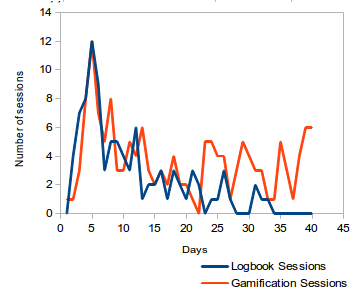
\includegraphics[width=0.5\textwidth]{Figures/scatter_daily_sessions.png}
    \rule{35em}{0.5pt}
  \caption{Average utilization of services and apps by the two groups of participants.}
  \label{figure:usagedailysessions}
\end{figure}\newline
There were two usage comparisons. In the first comparison, I contrasted usage in each day between the Logbook App and Gamified App by computing the daily total number of sessions from all users in a particular experimental condition. There were 41 days in total. Therefore, each day had the total number of sessions in each experimental condition as shown on Figure \ref{figure:usagedailysessions}. After the fourth week there was a decline in usage as the result of the learning effect. The decline was more apparent to users who where switched from gamification to logbook. I used ``\emph{Shapiro-Wilk Normality Test}''\footnote{http://sdittami.altervista.org/shapirotest/ShapiroTest.html} to test for normal distribution between logbook sessions and gamification sessions. The distribution of each of the two independent samples were not normal. An attempt to transform the data using transformation algorithms didn't yield to normal distributions. Therefore, I made a decision to use a non-parametric test called Mann-Whitney U Test. The number of sessions in Gamification condition were significantly higher than in Logbook condition as shown on Table \ref{table:usagedays}.
\begin{table}[h!]
  \begin{center}
    \caption{Daily usage comparison between Logbook and Gamified systems for 41 days}
    \label{table:usagedays}
	\begin{tabular}{|c|c|c|c|c|c|c|}
		\hline
		Groups&N&Rank Average&Sum Ranks&U&Z&P\\
		\hline
   		Logbook sessions&41&33.72&1701.5&\multirow{2}{*}{1159.5}&\multirow{2}{*}{-2.9538}& \multirow{2}{*}{0.00318}\\\cline{1-4} 
   		 		    Gamification sessions&41&49.28& 1701.5&&&\\
\hline
	\end{tabular}
  \end{center}
\end{table}
\newline 
The second comparison entailed contrasting `Logbook'' usage versus ``Gamification'' usage for each pair. I compared usage by counting both the number of days and total number sessions from each pair of users. Since the number of days and total sessions were relative to how many days users were exposed to a particular experimental condition, I divided the number of sessions with total days on which users were exposed to a particular experimental condition to get the ratio of days with respect to the total number of days and number of sessions per day. Therefore, comparison was based on a relative number and not an absolute. For instance, lets say pair one is from a LG group which they had access to a logbook system for 27 days and a gamified system for 14 days. Suppose the number of sessions in Logbook is 50 and the number of sessions in Gamified system is 30 then the relative number of sessions per day spent on logbook is 50 divide by 27 days and the relative number of session spent on  a gamified system is 30 divide by 27. Before comparing the two versions of the system on usage, I had to test if the differences of both the ratio of days and number of sessions per day between the two systems followed a normal distribution in order to identify a proper statistical test to use. The difference between logbook and gamification didn't have a normal distribution in both the ratio of days and number of sessions per day. I applied a natural logarithm transformation on the data and the difference of logs of both cases followed a normal distribution. 
\newline 
\begin{table}[h!]

  \begin{center}
    \caption{Usage comparison between Logbook and Gamified systems for 14 pairs of users}
    \label{table:usagewellness1}
	\begin{tabular}{|c|c|c|}
		\hline
		Log mean &Logbook App&Gamified App\\
		\hline
		 \multirow{2}{*}{Ratio of days}&M=0.16;SD=0.15&M=0.24 ;SD=0.18\\\cline{2-3} 

		 &\multicolumn{2}{|l|}{t(13)= 1.4927 ; p=0.1594 ; 95\% CI= -0.184 to 0.034} \\
\hline
   		 \multirow{2}{*}{ Number of sessions/day}&M=0.22 ;SD=0.22&M=0.36;SD=0.33\\\cline{2-3} 
		
		 &\multicolumn{2}{|l|}{t(13)=1.5519 ; p=0.1447 ; 95\% CI= -0.341 to 0.056} \\
\hline

	\end{tabular}
  \end{center}
\end{table}
\newline  
 
I carried out a paired student t-test on logarithmic transformed data.  On comparison of usage between a gamified system and logbook system, the former had a higher mean log of ratio of days  and mean log of number of sessions per day compared to the latter without statistical significance.
The results are shown on Table \ref{table:usagewellness1} above.
 
There were four pairs who faced hurdles on utilizing the app and this affected both their motivation and ability to participate or access the system. These pairs are listed on Table \ref{table:usageproblems}.\newline
\begin{table}[h!]
  \begin{center}
    \caption{Pairs with usability/technical problems that hinder their participation}
    \label{table:usageproblems}
	\begin{tabular}{|l|l|l|p{6cm}|}
		\hline
		&Pair&Experimental Sequence&Problem\\
		\hline
		1&Pair A&GL group &App not loading\\
		\hline
		2&Pair B&GL group&Lack of data bundles. \\
		\hline
		3&Pair C & LG group.& Pedometer never transmitted data to the server.\\
		\hline
		4&Pair D & LG group.& Pedometer stopped transmitting data to the server.\\
	\hline
	\end{tabular}
  \end{center}
\end{table}
\newline 
For \textbf{Pair A}, the app failed to load every time their intermediary user tried to use it. This pair had used the app for only two days  of which both days were during the gamification condition. What I observed from the house where this pair lived in is that there was a poor Internet signal hence the app was always failing to load most of the time. The second pair (\textbf{Pair B}), data was allocated to the wrong phone number at the beginning of experiments but they never reported on time. This pair had used the app for only three days of which both days were in gamification condition.   The last two pairs (\textbf{Pair C} and \textbf{Pair D}) both had their pedometers not transmitting steps data that were partially important in gamification for advancement of badges, and improvement of both the fish tank and the botanical garden. Pair C's pedometer never transmitted any readings to the server even in logbook condition.  Pair D's pedometer stopped transmitting steps data on the fourth week of running the experiments and this was before this particular user was switched to gamification condition. The two intermediary users from Pair C and Pair D were close friends. Although the pedometer never transmitted data in Pair C,an intermediary user from this pair continued to use the wellness app because of the informal comparison with an intermediary user from Pair D while they were still in logbook condition. The usage in Pair C and Pair D were both eleven days. Their drop out started during gamification condition. Pair C used the app for only three days and Pair D used it for only one day. Since gamification depended on transmission of steps to the server, pedometer problems affected Pair C and Pair D motivations to participate in gamification phase despite their efforts during logbook condition. The learning effect coupled with problems with their pedometers mediated their decrease in motivation to continue engage with the app.  An intermediary user from another pair in "LG" group who happened to live close to the Pair D and Pair C, shared her concerns about the rewards from the gamified app. This was during the endline interviews. This particular intermediary user didn't appreciate her advancement in badges because she admitted that her peers (the two intermediary users from Pair C and Pair D) did more efforts than her but they were not getting anything so she didn't understand why she was ahead of them. She was referring to their usage during logbook condition as they were both using the ``logbook App'' at the same time.  This proves that usability problems played a role to the some extent in demotivating participation in gamification condition  of intermediary users from Pair B and Pair C.

I repeated the above analysis on usage (Table \ref{table:usagewellness1}) without the pairs on Table \ref{table:usageproblems}. Therefore, the new analysis has only ten pairs of users. The results of the analysis are presented on Table\ref{table:usagewellness2}. A student t test demonstrated that the means log of both  the ratio of days 0.0183and number of sessions per day were significantly higher in the gamified system compared to the logbook system.
\newline 
\begin{table}[h!]
  \begin{center}
    \caption{Usage comparison between Logbook and Gamified systems for 11 pairs of users}
    \label{table:usagewellness2}
	\begin{tabular}{|c|c|c|}
		\hline
		Log mean &Logbook App&Gamified App\\
		\hline
		 \multirow{2}{*}{Ratio of days}&M=0.156;SD=0.141&M=0.285 ;SD=0.182\\\cline{2-3} 

		 &\multicolumn{2}{|l|}{t(9)= 2.3846 ; p=0.0409 ; 95\% CI= -0.252 to -0.066} \\
\hline
   		 \multirow{2}{*}{ Number of sessions/day}&M=0.201 ;SD=0.196&M=0.459;SD=0.336\\\cline{2-3} 
		
		 &\multicolumn{2}{|l|}{t(9)= 2.6593 ; p= 0.0261 ; 95\% CI=  -0.477 to -0.039 } \\
\hline
	\end{tabular}
  \end{center}
\end{table}
\newline  
Baseline data such as demographic information were not statistically sufficient to explain the above usage. There was an indication that male intermediaries had higher average number of sessions compared to female intermediaries as shown on Figure \ref{figure:usagegender}.  Also younger intermediaries had higher average number of sessions compared to the old ones as shown on Figure \ref{figure:usageage}. The aforementioned figures were for intermediaries from twelve pairs including Pair C and Pair D on Table \ref{table:usageproblems}. Pair A and Pair B were not considered as they terminated their usage on the first week of experiments. \newline
\begin{figure}[htbp]
  \centering
    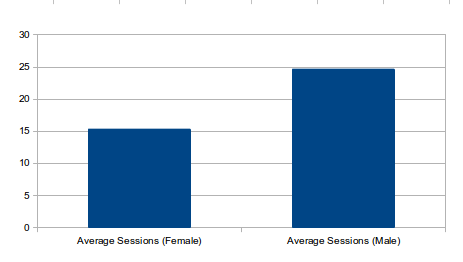
\includegraphics[width=0.5\textwidth]{Figures/session_gender.png}
    \rule{35em}{0.5pt}
  \caption{Average number of sessions between 6 male and 6 female intermediaries.}
  \label{figure:usageage}
\end{figure}
\begin{figure}[htbp]
  \centering
    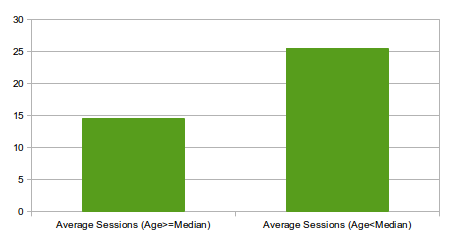
\includegraphics[width=0.5\textwidth]{Figures/session_age.png}
    \rule{35em}{0.5pt}
  \caption{Average number of sessions of 12 intermediaries between age\textgreater=Median(15.5) and age\textless Median(15.5) years.}
  \label{figure:usagegender}
\end{figure}\newline
\subsection{User Experience of Intermediaries}
User experience was analysed through IMI(Intrinsic Motivation Inventory) questionnaires and interviews. The first step was to examine how baseline intrinsic motivation and  demographic information such as age and gender influence user experience. From Figure \ref{figure:usageage} above, we saw that young intermediaries (age\textless median=15.5 years) appeared to have more number of sessions on average, but contrary to this trend is that, at baseline the average perceived enjoyment on helping with cellphone related tasks was higher in intermediaries with age\textgreater=median compared to intermediaries with age\textless median for the 12 intermediary users as shown on Figure \ref{figure:PE_HELP_Age}. 
\begin{figure}[htbp]
  \centering
    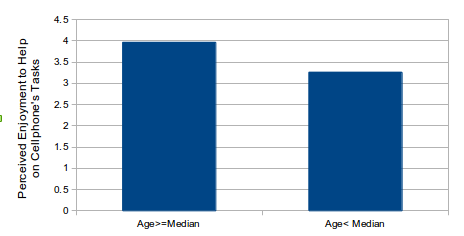
\includegraphics[width=0.5\textwidth]{Figures/PE_HELP_Age.png}
    \rule{35em}{0.5pt}
  \caption{Intermediaries' average perceived enjoyment to help others with cellphone tasks versus age group.}
  \label{figure:PE_HELP_Age}
\end{figure}\newline
I started by comparing perceived enjoyment by age at midline and endline of the 12 intermediary users (excluding users from Pair A and B since they terminated their usage too soon). Six intermediary users were below the median age of 15.5 while the remaining seven intermediary users were above the median age. More information on these two age groups is provided on Table \ref{table:agregroups}. We can see that both age groups have representatives from both experimental sequences (GL, and LG) and from both genders. Figure \ref{figure:PE_Interm_App} shows the averages of perceived enjoyment to use the family wellness app at midline and endline. The averages are higher on the intermediaries with age \textless median for both midline and endline points. \newline
\begin{table}[h!]
  \begin{center}
    \caption{Age groups of intermediary participants}
    \label{table:agregroups}
	\begin{tabular}{|c|L{3.2cm}|L{1cm}|L{2cm}|L{2cm}|L{1.6cm}|L{1.3cm}|}
    		\hline
         &\textbf{Age Groups}&\textbf{Total users}&\textbf{No. of GL sequence}&\textbf{No. of LG sequence}&\textbf{No. of Females}&\textbf{No. of Males}\\
         \hline
         1&Age \textgreater=15.5 years&6&3&3&2&4\\  
\hline
         2&Age \textless15.5 years&6&2&4&4&2\\  
\hline
	\end{tabular}
  \end{center}
\end{table}\newline 
\begin{figure}[htbp]
  \centering
    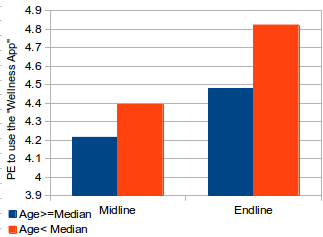
\includegraphics[width=0.5\textwidth]{Figures/PE_Interm_App.png}
    \rule{35em}{0.5pt}
  \caption{Intermediaries' average perceived enjoyment in using the app versus age group.}
  \label{figure:PE_Interm_App}
\end{figure}\newline
I observed the following factors that are important to user experience and their power in motivating intermediaries to interact with the app varied from pair to pair:
\begin{enumerate}
\item{\textbf{Self-monitoring task}}: The task itself of self-monitoring without rewards can spark interests of some intermediary users. This might be as the result of the novelty effect of visualization mechanisms. For instance one intermediary user who happened to be the youngest among all intermediaries reported the highest perceived enjoyment during logbook condition compared to other intermediary users. In addition it seems the phone also had an impact on triggering her interests.
\item{\textbf{Informal comparisons}}: Comparison on steps graphs can be another source motivation. For intermediaries who were close, they did this form of informal comparison. In the absence of gamification, still intermediaries thought that they were competing with other therefore those who were close had face to face interactions of where they did comparison with one another. 
\item{\textbf{Gamification comparison}}: This kind of comparison increased the number of times intermediary user checked the app. However, not all intermediaries had enjoyed using the gamification condition.
\end{enumerate}
This suggests the task of helping might be less interesting to younger intermediaries provided that there are no motivational affordances.\newline
The IMI questionnaire that assessed intrinsic motivation in using the ``The Family Wellness App'' had four sub-scales which where perceived competence, perceived autonomy,perceived enjoyment, and perceived relatedness.  
Our hypotheses of interest for intermediaries were
\begin{enumerate}
\item{Hypothesis 1}
\begin{itemize}
\item{H\SB{0}}:There is no difference in perceived competence in using  between a Logbook app and Gamified app
\item{H\SB{A}}:There is a difference in perceived competence in using  between a Logbook app and Gamified app
\end{itemize}
\item{Hypothesis 1}
\begin{itemize}
\item{H\SB{0}}:There is no difference in perceived autonomy in using between a Logbook app and Gamified app
\item{H\SB{A}}:There is a difference in perceived autonomy between a Logbook app and Gamified app
\end{itemize}
\item{Hypothesis 3}
\begin{itemize}
\item{H\SB{0}}:There is no difference in perceived enjoyment in using  between a Logbook app and Gamified app
\item{H\SB{A}}:There is a difference in perceived enjoyment in using between a Logbook app and Gamified app
\end{itemize}
\item{Hypothesis 4}
\begin{itemize}
\item{H\SB{0}}:There is no difference in perceived relatedness in using between a Logbook app and Gamified app
\item{H\SB{A}}:There is a difference in perceived relatedness in using between a Logbook app and Gamified app
\end{itemize}
\end{enumerate}

The ``Gamified App'' was designed in such a way that a pair will earn rewards based on usage points and the average number of steps walked by a beneficiary participant who is a member of the pair. The purpose of rewards was to foster users' intrinsic experiences such as competitiveness and a sense of autonomy which are predictors of intrinsic motivation. Reward depended on four parameters and these were the number of steps walked by a beneficiary user, the number of days the app has been used by an intermediary to either to record meals or to view feedback on meals, points, steps, gardens, etc. On comparison of competitiveness and autonomy of between gamified condition and logbook condition, there six intermediaries that were excluded.\newline
The first four users are from the pairs on Table \ref{table:usageproblems} above who were listed as having technical/usability problems hence they didn't stand a better chance to participate fully on the experiments.  Apart from the four intermediary users, there was  a very intriguing phenomenon from other two intermediary users from \textbf{Pair E} and \textbf{Pair F} as mentioned on Table \ref{table:negexprnce}. The two intermediary users had used the app more often in gamification condition  compared to when they were in logbook condition but had reported both lower scores in perceived enjoyment, and perceived competence when in gamified condition compared to when they were in logbook condition. Two of these intermediary users were  in LG and GL groups respectively. I examined the performance of these two users in gamification rewards and discovered that two users never managed to make any progress in attaining a single reward despite their efforts in using the ``Gamified App''.This harmed both their perceived enjoyment and perceived competence to use the "Family Wellness App" while in gamification condition. One of these two intermediary participants sent an SMS to the researcher asking what he was supposed to do in order to advance in badges and he was informed that all the information was specified in their given user manual. In addition, SMS reminders were sent out to all intermediaries to inform them of how far they have gone in achieving rewards and what is remaining in terms of usage and steps in order for them to reach the next badge. Their beneficiary participants were not walking enough steps despite the fact that these intermediaries had put  efforts in engaging with the App. One beneficiary who was working with one of these intermediary users also reported in interviews that there was always a contention with her intermediary when this beneficiary wanted to see what was going in the app as the intermediary was not voluntarily willing to help some of the time.\newline
\begin{table}
  \begin{center}
    \caption{Pairs affected by poor design of gamification}
    \label{table:negexprnce}
	\begin{tabular}{|l|l|l|p{6cm}|}
		\hline
		&Pair&Experimental Sequence&Challenge\\
		\hline
		1&Pair E&LG group & The beneficiary participant was not walking enough steps hence impacted performance in gamification\\
		\hline
		2&Pair D & LG group.& Same as above.\\
	\hline
	\end{tabular}
  \end{center}
\end{table}
\newline 
Therefore, on comparison between Logbook and Gamification, I excluded a total of six intermediary users on perceived competence, perceived enjoyment, and perceived autonomy as these three sub-scales are directly linked to intrinsic motivation. Four out of those  intermediaries had usability/technical problems as mentioned above and this might have impacted their user experience while the remaining two had a negative experience as the result of failure of our gamification design to match challenges with abilities. i.e. efforts of beneficiaries differed hence challenges should have matched with individual abilities of beneficiaries within pairs. When challenges are too difficult as they don't match users' skills, end users can become demotivated \citep{zhang2008motivational}. As result only eight intermediary users were considered in the main sub scales of intrinsic motivation (autonomy, competence, and enjoyment). 
 
I started with comparison on perceived competence, perceived autonomy, and perceived enjoyment between the ``Logbook App''  and the ``Gamified App''. The distribution of the differences of all the scores from the three aforementioned sub-scales, followed a normal distribution hence met a condition for using a paired student t-test. The results of the paired student t-test on the three IMI sub-scales scores of the nine intermediaries are shown on Table \ref{table:imiwellnessinterm}. Perceived competence of intermediaries in using the ``Family Wellness App'' was significantly higher in the gamified condition than in the logbook condition in eight intermediaries that were analysed. Perceived autonomy,and perceived enjoyment were both not different between gamification condition and logbook condition. \newline
\begin{table}[h!]
  \begin{center}
    \caption{Comparison of eight intermediaries' scores on sub-scales of competence, autonomy, and enjoyment in using the ``Family Wellness App}
    \label{table:imiwellnessinterm}
	\begin{tabular}{|c|c|c|}
		\hline
		Mean &Logbook App&Gamified App\\
		\hline
		 \multirow{2}{*}{Perceived competence}&M=5.38;SD=0.91&M=6.04;SD=0.7\\\cline{2-3} 

		 &\multicolumn{2}{|l|}{t(7)=3.0619 ; p=0.0183 ; 95\% CI= -1.176 to -0.151   } \\
\hline
		 \multirow{2}{*}{Perceived autonomy}&M=4.5; SD=1.27&M=4.92; SD=1.22\\\cline{2-3} 

		 &\multicolumn{2}{|l|}{t(7)=1.0584; p= 0.3250; 95\% CI= -1.342 to 0.512  } \\
\hline
		 \multirow{2}{*}{Perceived enjoyment}&M=4.29; SD=1.24&M=4.63; SD=1.45\\\cline{2-3} 

		 &\multicolumn{2}{|l|}{t(7)= 0.7071 ; p=0.5 ; 95\% CI=  -1.448 to 0.781 } \\
\hline
	\end{tabular}
  \end{center}
\end{table}
\newline  
All fourteen pairs were considered in perceived relatedness including pairs that were excluded on results of Table \ref{table:imiwellnessinterm}. The reason of why we considered all pairs is that despite of problems faced by some users,seeing other users on the app or just receiving messages  or face to face interactions were means on which users could relate to each other.  Therefore, all users were interacting with one another whether through the app,receiving of text messages or by having face to face conversations. For instance during gamification, a text message mentioning the users who are on top three list was sent in after every two days. All intermediary users received these text messages. Also there are intermediary users who had face to face interactions to discuss what was going with regard to usage of the ``Family Wellness App''.\newline
Comparison on perceived relatedness of between the logbook and gamified conditions is shown on Table \ref{table:imiwellnessinterm2}. There was no difference in relatedness in between logbook condition and gamified condition although the average perceived relatedness was higher in gamification condition\newline 
\begin{table}[h!]
  \begin{center}
    \caption{Comparison of fourteen intermediaries' scores on perceived relatedness in using the ``Family Wellness App}
    \label{table:imiwellnessinterm2}
	\begin{tabular}{|c|c|c|}
		\hline
		Mean &Logbook App&Gamified App\\
		\hline
		 \multirow{2}{*}{Perceived relatedness}&M=4.20; SD=0.59&M=4.5; SD=1.04\\\cline{2-3} 
		 &\multicolumn{2}{|l|}{t(13)= 1.5046; p=0.1563; 95\% CI= -0.725 to 0.13} \\
\hline
	\end{tabular}
  \end{center}
\end{table}
\newline
\begin{flushright}

\end{flushright}

